\documentclass[preprint,12pt,aps,pra,showkeys,amsmath,amssymb,superscriptaddress,floatfix]{revtex4-2}
\usepackage[T1]{fontenc}
\usepackage[utf8]{inputenc}
\usepackage{amsmath,amssymb,amsthm,mathtools,mathrsfs}
\usepackage{microtype,booktabs,enumitem}
\usepackage{xcolor,tikz,etoolbox}
\usepackage[skins,breakable]{tcolorbox}
\usepackage{needspace}
% Keep diagram geometry independent of REVTeX preprint body spacing.
\AtBeginEnvironment{tikzpicture}{\linespread{1}\selectfont}
\usetikzlibrary{arrows.meta,positioning,calc,fit,decorations.pathreplacing}
\usepackage{graphicx}
\usepackage{hyperref}

\definecolor{MMBlue}{RGB}{0,82,155}
\definecolor{MMOrange}{RGB}{200,80,0}
\tikzset{
 mmnode/.style={draw=MMBlue,rounded corners=2pt,fill=MMBlue!4,align=left,execute at begin node={\raggedright},text width=5cm,font=\fontsize{10}{12}\selectfont,inner sep=6pt},
 mmimport/.style={mmnode,draw=black!65,fill=black!4},
 mmcandidate/.style={mmnode,draw=MMOrange,dashed,fill=MMOrange!5},
 mmrejected/.style={mmnode,draw=black,densely dotted,fill=black!8},
 mmproof/.style={->,thick,MMBlue},
 mmflow/.style={->,semithick,black!70},
 mmrepair/.style={->,dashed,thick,MMOrange},
 mmcandidatearrow/.style={->,dashed,semithick,MMOrange},
 mmnote/.style={font=\scriptsize,fill=white,inner sep=2pt,align=center}}

\usepackage[section]{placeins}
\setlength{\emergencystretch}{3em}
\setlist{itemsep=3pt,topsep=4pt}
\newtheorem{theorem}{Theorem}[section]
\newtheorem{proposition}[theorem]{Proposition}
\newtheorem{lemma}[theorem]{Lemma}
\newtheorem{corollary}[theorem]{Corollary}
\theoremstyle{definition}
\newtheorem{definition}[theorem]{Definition}
\newtheorem{example}[theorem]{Example}
\theoremstyle{remark}
\newtheorem{remark}[theorem]{Remark}
% Avoid isolated statement headings and single-line paragraph fragments.
\BeforeBeginEnvironment{theorem}{\Needspace{6\baselineskip}}
\BeforeBeginEnvironment{definition}{\Needspace{5\baselineskip}}
\BeforeBeginEnvironment{proposition}{\Needspace{5\baselineskip}}
\BeforeBeginEnvironment{lemma}{\Needspace{5\baselineskip}}
\BeforeBeginEnvironment{corollary}{\Needspace{5\baselineskip}}
\clubpenalty=5000
\widowpenalty=5000
\newcommand{\R}{\mathbb R}\newcommand{\Z}{\mathbb Z}\newcommand{\N}{\mathbb N}
\newcommand{\Pa}{\operatorname{Pa}}\newcommand{\Desc}{\operatorname{Desc}}
\newcommand{\cl}{\operatorname{cl}}\newcommand{\cost}{\operatorname{cost}}
\newcommand{\status}{\operatorname{status}}
% Faculty cards: a visual rail groups the five faculties within one agent.
% The rail has no arrowhead and does not represent a proof dependency.
\newcommand{\mmfacultybadge}[1]{%
 \node[circle,draw=MMBlue,line width=1pt,fill=white,
 minimum size=7mm,inner sep=0pt,font=\sffamily\small\bfseries,text=MMBlue]
 at ([xshift=15pt,yshift=-15pt]frame.north west) {#1};}
\newcommand{\mmfacultyrail}{%
 \draw[MMBlue!80,line width=1pt]
 ([xshift=15pt,yshift=2pt]frame.north west)--
 ([xshift=15pt,yshift=-2pt]frame.south west);}
\newtcolorbox{mmfacultybox}[2]{enhanced,breakable,
 colback=MMBlue!4,colframe=MMBlue!4,boxrule=0pt,arc=3pt,
 left=39pt,right=9pt,top=4pt,bottom=4pt,
 before skip=2pt,after skip=2pt,
 fontupper=\small\linespread{1.1}\selectfont,
 overlay unbroken={\mmfacultyrail\mmfacultybadge{#1}},
 overlay first={\mmfacultyrail\mmfacultybadge{#1}},
 overlay middle={\mmfacultyrail},overlay last={\mmfacultyrail}}
\newcommand{\mmfaculty}[3]{%
 \begin{mmfacultybox}{#1}{#2}
 {\sffamily\bfseries\color{MMBlue}#2}\par\smallskip #3
 \end{mmfacultybox}}
\newcommand{\agent}[9]{%
 \Needspace{8\baselineskip}
 \subsubsection{#1}
 \noindent\textbf{Object.} #2\par
 \noindent\textbf{Role.} #3\par\smallskip
 \mmfaculty{E}{Ego}{#4}
 \mmfaculty{M}{Memory}{#5}
 \mmfaculty{I}{Intellect}{#6}
 \mmfaculty{S}{Sense}{#7}
 \mmfaculty{A}{Action}{#8}
 \smallskip\noindent #9\par}

\usepackage{longtable,array,calc}
\providecommand{\tightlist}{\setlength{\itemsep}{2pt}\setlength{\parskip}{0pt}}
\makeatletter
\def\frontmatter@abstract@produce{\par\addvspace{\frontmatter@preabstractspace}%
\begingroup\prep@absbox\unvbox\absbox\post@absbox\endgroup
\addvspace{\frontmatter@postabstractspace}}
\makeatother
\newcommand{\field}[2]{\par\smallskip\noindent\textbf{#1.} #2\par}
\setlength{\emergencystretch}{5em}
\AtBeginEnvironment{verbatim}{\small\linespread{1.0}\selectfont}


\hypersetup{colorlinks=true,linkcolor=MMBlue,urlcolor=MMBlue,pdfauthor={Dibakar Sigdel}}

\begin{document}

\title{Fundamental Group of the Circle\\[4pt]\large An End-to-End Meta-Math Walkthrough}

\author{Dibakar Sigdel}

\affiliation{Mindverse Computing LLC, Lynnwood, WA 98087, USA}

\date{October 2026}

\begin{abstract}

A complete authored walkthrough of fundamental group of the circle, with
explicit mathematical contracts, local verification gates, and reusable
exports. The report presents the target theorem, declared imports, a
dependency graph, five-faculty node contracts, a continuous proof, a
worked example, and a hypothesis-repair audit. It is an authored
mathematical exposition, not a deployed-agent transcript or a formal
proof-assistant certificate.

\end{abstract}\maketitle\linespread{1.12}\selectfont

\noindent\textbf{AT-01 / Algebraic Topology / Report v1}

\section{Target and import contract}

\begin{theorem}

Prove \(\pi_1(S^1,1)\cong\mathbb Z\) using the covering map
\(p:\mathbb R\to S^1\), \(p(t)=e^{2\pi it}\).

\end{theorem}

\subsection{Foundations and permitted imports}

Use the covering \(p:R\to S^{1}\), \(p(t)=e^{(2\pi it)}\). Import path
lifting with prescribed initial value and homotopy lifting for a
covering map: a path, or a homotopy of paths, has a unique continuous
lift after an initial lift is fixed. Here evenly covered arcs supply the
local inverses, and compact subdivision supplies global lifting. Based
loops start/end at 1; their chosen lifts start at 0.

\clearpage\section{Node interaction workflow}

\begin{center}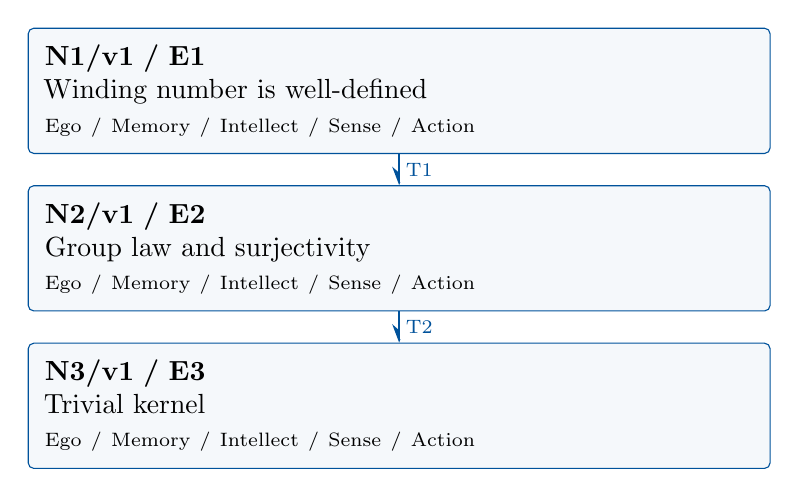
\begin{tikzpicture}[>=Stealth,x=1cm,y=1cm]

\node[mmnode,text width=9cm,minimum height=1.25cm] (N1) at (0,0.0) {\textbf{N1/v1 / E1}\\Winding number is well-defined\\{\scriptsize Ego / Memory / Intellect / Sense / Action}};

\node[mmnode,text width=9cm,minimum height=1.25cm] (N2) at (0,-2.0) {\textbf{N2/v1 / E2}\\Group law and surjectivity\\{\scriptsize Ego / Memory / Intellect / Sense / Action}};

\node[mmnode,text width=9cm,minimum height=1.25cm] (N3) at (0,-4.0) {\textbf{N3/v1 / E3}\\Trivial kernel\\{\scriptsize Ego / Memory / Intellect / Sense / Action}};

\draw[mmproof] (N1.south) -- node[mmnote,right] {T1} (N2.north);

\draw[mmproof] (N2.south) -- node[mmnote,right] {T2} (N3.north);

\end{tikzpicture}\end{center}

Each box is one mathematical agent containing all five faculties. Blue
arrows carry the versioned exports listed below. The layout gives a
reading order; only drawn arrows assert dependencies. Diagnostic repair
is separate from the proof DAG.

\subsection{Versioned evidence-transfer ledger}

\begingroup\small\linespread{1.05}\selectfont

\Needspace{5\baselineskip}\field{T1: N1/E1/v1 to N2}{An integer winding invariant on \(\pi _{1}(S^{1},1)\).}

\field{Receiving activity}{N2: Group law and surjectivity}

\field{Compatibility}{Use the same mathematical objects and hypotheses as the source export.
Receiving contract: Two lifted loops and their endpoints; prior exports
E1/v1}

\Needspace{5\baselineskip}\field{T2: N2/E2/v1 to N3}{A surjective homomorphism \(w:\pi _{1}(S^{1},1)\to Z\).}

\field{Receiving activity}{N3: Trivial kernel}

\field{Compatibility}{Use the same mathematical objects and hypotheses as the source export.
Receiving contract: A lift with endpoint0; prior exports E2/v1}

\endgroup

\clearpage\section{Agent roles and five-faculty activities}\begingroup\small\linespread{1.05}\selectfont\setlist{itemsep=1pt,topsep=2pt}

\subsection{N1/v1: Winding number is well-defined}

\field{Object and role}{Read the integer endpoint and audit based homotopies.}

\field{Inputs}{A based loop \(\alpha\) and its lift \(\widetilde{\alpha}\);
foundational imports stated in §1}

\mmfaculty{E}{Ego}{Own E1/v1: An integer winding invariant on \(\pi _{1}(S^{1},1)\).}

\mmfaculty{M}{Memory}{Retain A based loop \(\alpha\) and its lift \(\widetilde{\alpha}\);
foundational imports stated in §1; keep their assumptions and versions
attached.}

\mmfaculty{I}{Intellect}{Read the integer endpoint and audit based homotopies.}

\mmfaculty{S}{Sense}{The basepoint must remain fixed during the homotopy.}

\mmfaculty{A}{Action}{Carry out the numbered deductions and publish E1/v1 together with its
hypotheses and proof location.}

\smallskip\noindent\textbf{Numbered mathematical activities}

\begin{enumerate}[label=N1.\arabic*,leftmargin=3.4em]

\item Since \(p(\widetilde{\alpha}(1))=1\), the endpoint lies in Z.

\item For a based homotopy, its lift has initial endpoint0 throughout; the
terminal lifted endpoint is a continuous integer-valued function of the
homotopy parameter, hence constant.

\item Thus \(w([\alpha ])=\widetilde{\alpha}(1)\) depends only on the based
homotopy class.

\end{enumerate}

\field{Export E1/v1}{An integer winding invariant on \(\pi _{1}(S^{1},1)\).}

\field{Acceptance gate}{The basepoint must remain fixed during the homotopy. Publish only after
checking every displayed deduction.}

\field{Targeted repair}{If the check fails, revise N1: The basepoint must remain fixed during
the homotopy. Recheck dependent nodes N2, N3.}

\clearpage

\subsection{N2/v1: Group law and surjectivity}

\field{Object and role}{Translate the second lift before concatenating.}

\field{Inputs}{Two lifted loops and their endpoints; prior exports E1/v1}

\mmfaculty{E}{Ego}{Own E2/v1: A surjective homomorphism \(w:\pi _{1}(S^{1},1)\to Z\).}

\mmfaculty{M}{Memory}{Retain Two lifted loops and their endpoints; prior exports E1/v1; keep
their assumptions and versions attached.}

\mmfaculty{I}{Intellect}{Translate the second lift before concatenating.}

\mmfaculty{S}{Sense}{Concatenating two lifts both based at 0 would create a discontinuity
unless the first winding is 0.}

\mmfaculty{A}{Action}{Carry out the numbered deductions and publish E2/v1 together with its
hypotheses and proof location.}

\smallskip\noindent\textbf{Numbered mathematical activities}

\begin{enumerate}[label=N2.\arabic*,leftmargin=3.4em]

\item If lifts of \(\alpha\) and \(\beta\) end at m andn, a lift of the
concatenation is the lift of \(\alpha\) followed by the lift of
\(\beta\) translated bym; its endpoint is m+n.

\item Hencew is a homomorphism.

\item For each \(n\in Z\) the loop \(\alpha _n(t)=e^{(2\pi int)}\) has liftnt
and windingn, proving surjectivity.

\end{enumerate}

\field{Export E2/v1}{A surjective homomorphism \(w:\pi _{1}(S^{1},1)\to Z\).}

\field{Acceptance gate}{Concatenating two lifts both based at 0 would create a discontinuity
unless the first winding is 0. Publish only after checking every
displayed deduction.}

\field{Targeted repair}{If the check fails, revise N2: Concatenating two lifts both based at 0
would create a discontinuity unless the first winding is 0. Recheck
dependent nodes N3.}

\clearpage

\subsection{N3/v1: Trivial kernel}

\field{Object and role}{Contract the closed lifted loop and project.}

\field{Inputs}{A lift with endpoint0; prior exports E2/v1}

\mmfaculty{E}{Ego}{Own E3/v1: The fundamental group of the circle with its explicit winding
isomorphism.}

\mmfaculty{M}{Memory}{Retain A lift with endpoint0; prior exports E2/v1; keep their
assumptions and versions attached.}

\mmfaculty{I}{Intellect}{Contract the closed lifted loop and project.}

\mmfaculty{S}{Sense}{A projected contraction must preserve both loop endpoints.}

\mmfaculty{A}{Action}{Carry out the numbered deductions and publish E3/v1 together with its
hypotheses and proof location.}

\smallskip\noindent\textbf{Numbered mathematical activities}

\begin{enumerate}[label=N3.\arabic*,leftmargin=3.4em]

\item If \(w([\alpha ])=0\) then
\(\widetilde{\alpha}(0)=\widetilde{\alpha}(1)=0\).

\item The homotopy \(H(s,t)=p((1-s)\widetilde{\alpha}(t))\) is continuous,
remains based at 1 at both endpoints, equals \(\alpha\) when \(s=0\),
and is the constant loop when \(s=1\).

\item Thus \(\alpha\) is null-homotopic.

\item The kernel is trivial, so the surjective homomorphism is injective and
\(\pi _{1}(S^{1},1)\cong Z\).

\end{enumerate}

\field{Export E3/v1}{The fundamental group of the circle with its explicit winding
isomorphism.}

\field{Acceptance gate}{A projected contraction must preserve both loop endpoints. Publish only
after checking every displayed deduction.}

\field{Targeted repair}{If the check fails, revise N3: A projected contraction must preserve
both loop endpoints. Withhold this terminal result until its gate
passes.}

\endgroup\clearpage\section{Continuous mathematical proof}\label{sec:proof}

Read these steps in order as one proof; the diagram is optional.
Numbered activities identify the specific constructions and deductions
owned by each node.

\subsection{§4.N1 --- Winding number is
well-defined}\label{n1-winding-number-is-well-defined}

For a based loop \(\alpha\), let \(\widetilde\alpha\) be its unique lift
starting at zero.

\begin{enumerate}
\def\labelenumi{\arabic{enumi}.}
\item
  Since \(p(\widetilde{\alpha}(1))=1\), the endpoint lies in Z.
\item
  For a based homotopy, its lift has initial endpoint0 throughout; the
  terminal lifted endpoint is a continuous integer-valued function of
  the homotopy parameter, hence constant.
\item
  Thus \(w([\alpha ])=\widetilde{\alpha}(1)\) depends only on the based
  homotopy class.
\end{enumerate}

\subsection{§4.N2 --- Group law and
surjectivity}\label{n2-group-law-and-surjectivity}

\begin{enumerate}
\def\labelenumi{\arabic{enumi}.}
\item
  If lifts of \(\alpha\) and \(\beta\) end at m andn, a lift of the
  concatenation is the lift of \(\alpha\) followed by the lift of
  \(\beta\) translated bym; its endpoint is m+n.
\item
  Hencew is a homomorphism.
\item
  For each \(n\in Z\) the loop \(\alpha _n(t)=e^{(2\pi int)}\) has
  liftnt and windingn, proving surjectivity.
\end{enumerate}

\subsection{§4.N3 --- Trivial kernel}\label{n3-trivial-kernel}

\begin{enumerate}
\def\labelenumi{\arabic{enumi}.}
\item
  If \(w([\alpha ])=0\) then
  \(\widetilde{\alpha}(0)=\widetilde{\alpha}(1)=0\).
\item
  The homotopy \(H(s,t)=p((1-s)\widetilde{\alpha}(t))\) is continuous,
  remains based at 1 at both endpoints, equals \(\alpha\) when \(s=0\),
  and is the constant loop when \(s=1\).
\item
  Thus \(\alpha\) is null-homotopic.
\item
  The kernel is trivial, so the surjective homomorphism is injective and
  \(\pi _{1}(S^{1},1)\cong Z\).
\end{enumerate}

\hfill$\square$

\section{Worked orchestration}

The loop \(e^{(6\pi it)}\) has lift3t and winding3. Reversing it gives
\(-3\); concatenating it with \(e^{(-4\pi it)}\) gives winding1. The
covering itself identifies endpoint changes rather than relying on a
picture of turns.

\subsection{Boundary and hypothesis audit}

An open path ending at \(-1\) lifts to an endpoint in 1/2+Z, notZ, so it
does not define this loop invariant. Sense checks the endpoint and
based-homotopy conditions before exporting an integer.

\section{Illustrative failure and repair}

The following is an authored diagnostic scenario. Changed assumptions
define a new contract; they do not retroactively prove the original
statement.

\subsection{Failure and correction}
This is an authored teaching trace, not a recorded agent run.

\begin{enumerate}
\def\labelenumi{\arabic{enumi}.}
\tightlist
\item
  \textbf{Ego \(\to\) Memory:} register the §1 theorem, imports, and
  requested exports before beginning the proof.
\item
  \textbf{Intellect \(\to\) Action:} choose the bridges in §3 and carry
  out the numbered activities in §4; transmit only established E-exports
  along the §2 DAG.
\item
  \textbf{Sense \(\to\) responsible node:} test the specific
  boundary/failure in §5 and the node's individual audit. A failing
  candidate is withheld; downstream nodes may not use it.
\item
  \textbf{Memory + Intellect:} identify whether the error is an omitted
  condition, an invalid inference, or an attempted extension beyond the
  theorem. Restore the exact contract or explicitly state a different
  one.
\item
  \textbf{Action:} redo the affected mathematical activity using the
  repaired condition or inference. Recheck consuming nodes, rather than
  feeding their conclusions back as premises.
\item
  \textbf{Ego:} publish only the supported export with its assumptions
  and proof location. A hypothetical revised export is v2; the written
  proof here is the v1 exposition, not a claim that this repair was
  executed.
\end{enumerate}

\subsection{Hypothesis boundary}
An open path ending at \(-1\) lifts to an endpoint in 1/2+Z, notZ, so it
does not define this loop invariant. Sense checks the endpoint and
based-homotopy conditions before exporting an integer.

\subsection{Version and recheck}
Treat any changed assumption as a new contract. Recheck the revised
export and all of its descendants. A backward diagnostic never
establishes an earlier theorem. This is an authored teaching trace, not
an execution log.

\par\medskip\begingroup\small\linespread{1.0}\selectfont\noindent\textbf{Provenance.} This authored proof is complete relative to its declared imports. Reuse
each export with its assumptions, proof, and version. The original
Markdown remains available for comparison.
\par\endgroup

\par\smallskip\begingroup\small\linespread{1.0}\selectfont\noindent\textbf{Further reading.} \begin{itemize}
\tightlist
\item
  \href{https://pi.math.cornell.edu/~hatcher/AT/AT.pdf}{Allen Hatcher,
  Algebraic Topology: covering spaces, cellular homology, and cap
  products}.
\end{itemize}\par\endgroup

\end{document}
